% -----------------------------------------------------------
% DMA Discrete Mathematics — Comprehensive Practice Exam
% Compile with: xelatex exam.tex
% -----------------------------------------------------------
\documentclass[11pt,a4paper,fontset=mac]{ctexart}

% ---- Packages ----
\usepackage{amsmath,amssymb,amsthm}
\usepackage{geometry}
\geometry{margin=2.2cm}
\usepackage{array,booktabs,multirow}
\usepackage{enumitem}
\usepackage{xcolor}
\usepackage{fancyhdr}
\usepackage[colorlinks=true,linkcolor=blue]{hyperref}
\usepackage{tikz}

% ---- Page style ----
\pagestyle{fancy}
\fancyhf{}
\fancyhead[L]{\small DMA 离散数学}
\fancyhead[C]{\small 摸底考试卷}
\fancyhead[R]{\small 满分 100 | 90 分钟}
\fancyfoot[C]{\thepage}
\renewcommand{\headrulewidth}{0.4pt}

% ---- Paragraph spacing ----
\setlength{\parskip}{0.6ex}
\setlength{\parindent}{0pt}

% ---- Custom commands ----
\newcommand{\tfblank}{$\square$}
\newcommand{\question}[1]{\textbf{Q#1}.}
\newcommand{\ans}[1]{\textbf{#1}}

% ---- Document ----
\begin{document}

% ============================================================
\noindent\hrulefill
\begin{center}
  {\LARGE\bfseries DMA 离散数学 摸底考试卷}\\[4pt]
  {\large 考试范围：Ch1--6, Ch8--11 + Network Flow}
\end{center}
\hrulefill

\vspace{1em}
\noindent\textbf{姓名：}\underline{\hspace{4cm}}\hfill
\textbf{学号：}\underline{\hspace{4cm}}\hfill
\textbf{得分：}\underline{\hspace{2cm}}

\vspace{1em}
\begin{tabular}{ll}
  \textbf{满分} & 100 分 \\
  \textbf{时间} & 90 分钟 \\
  \textbf{Part 1} & 30\% \;--\; True/False（答对 $+3$，空白 $0$，答错 $-1$）\\
  \textbf{Part 2} & 40\% \;--\; 简答题 \\
  \textbf{Part 3} & 30\% \;--\; 综合题
\end{tabular}

% ============================================================
\section*{Part 1: True/False (30\%)}

\noindent\textbf{评分规则：}答对 $+3$ 分，空白 $0$ 分，答错 $-1$ 分（倒扣制）。
请在每题后的方框中填入 \texttt{T}（真）或 \texttt{F}（假）。

% ----------------------------------------------------------
\subsection*{Ch1\;\; Logic \& Proofs}

\question{1}  Let $P(x,y)$ be a predicate. Then
$\forall x\,\exists y\,P(x,y) \equiv \exists y\,\forall x\,P(x,y)$.
\hfill\tfblank

\question{2}  The negation of $\forall x\,(P(x)\to Q(x))$ is
$\exists x\,(P(x)\land\neg Q(x))$.
\hfill\tfblank

\question{3}  $(p\to q)\land(p\to r)\equiv p\to(q\land r)$.
\hfill\tfblank

% ----------------------------------------------------------
\subsection*{Ch2\;\; Sets \& Functions}

\question{4}  $|A\times B| = |A|\cdot|B|$ for any finite sets $A$ and $B$.
\hfill\tfblank

\question{5}  If $f:A\to B$ and $g:B\to C$ are both injective, then
$g\circ f$ is injective.
\hfill\tfblank

\question{6}  The set of all finite subsets of $\mathbb{N}$ is countable.
\hfill\tfblank

% ----------------------------------------------------------
\subsection*{Ch3\;\; Algorithms}

\question{7}  If $f(n)=3n^{2}+2n+1$, then $f(n)=\Theta(n^{2})$.
\hfill\tfblank

\question{8}  $n! = O(2^{n})$.
\hfill\tfblank

% ----------------------------------------------------------
\subsection*{Ch4\;\; Number Theory}

\question{9}  If $a\equiv b\pmod m$ and $c\equiv d\pmod m$, then
$ac\equiv bd\pmod m$.
\hfill\tfblank

\question{10}  $\gcd(a,b)\cdot\operatorname{lcm}(a,b)=ab$ for all positive
integers $a,b$.
\hfill\tfblank

% ----------------------------------------------------------
\subsection*{Ch5\;\; Induction}

\question{11}  The Well-Ordering Principle is equivalent to the Principle
of Mathematical Induction.
\hfill\tfblank

\question{12}  In strong induction, to prove $P(n)$ we assume $P(k)$ is
true for all $k<n$, not just $P(n-1)$.
\hfill\tfblank

% ----------------------------------------------------------
\subsection*{Ch6\;\; Counting}

\question{13}  $C(n,r)=P(n,r)/r!$ for all $0\le r\le n$.
\hfill\tfblank

\question{14}  By the pigeonhole principle, among any 13 people at least
2 were born in the same month.
\hfill\tfblank

% ----------------------------------------------------------
\subsection*{Ch8\;\; Recurrence Relations}

\question{15}  The characteristic equation of
$a_n = 3a_{n-1}-2a_{n-2}$ has roots $1$ and $2$.
\hfill\tfblank

\question{16}  The number of derangements of $n$ objects is approximately
$n!/e$.
\hfill\tfblank

% ----------------------------------------------------------
\subsection*{Ch9\;\; Relations}

\question{17}  Every equivalence relation on a set $A$ partitions $A$.
\hfill\tfblank

\question{18}  A relation that is symmetric and transitive must also be
reflexive.
\hfill\tfblank

% ----------------------------------------------------------
\subsection*{Ch10\;\; Graphs}

\question{19}  $K_{5}$ is a planar graph.
\hfill\tfblank

\question{20}  A connected multigraph has an Euler circuit iff every
vertex has even degree.
\hfill\tfblank

\question{21}  The chromatic number of a bipartite graph is at most $2$.
\hfill\tfblank

\question{22}  By the Handshaking Theorem, every graph has an even number
of vertices of odd degree.
\hfill\tfblank

% ----------------------------------------------------------
\subsection*{Ch11\;\; Trees}

\question{23}  Every tree with $n$ vertices has exactly $n-1$ edges.
\hfill\tfblank

\question{24}  In a full binary tree, the number of leaves equals the
number of internal vertices plus $1$.
\hfill\tfblank

% ----------------------------------------------------------
\subsection*{Network Flow}

\question{25}  By the Max-Flow Min-Cut Theorem, the value of a maximum
flow equals the capacity of a minimum cut.
\hfill\tfblank

% ============================================================
\section*{Part 2: Short Problems (40\%)}

% ----------------------------------------------------------
\subsection*{Ch1 -- Logic (6\%)}

\question{26}  Write an equivalent proposition of $p\oplus q$ using only
the NAND operator $\mid$.\bigskip

% ----------------------------------------------------------
\subsection*{Ch2 -- Sets (6\%)}

\question{27}  Let $A=\{1,2,3\}$, $B=\{2,3,4\}$. Compute:
\begin{enumerate}[label=(\alph*)]
  \item $A\oplus B$ (symmetric difference)
  \item $\mathcal{P}(A\cap B)$ (power set)
\end{enumerate}
\bigskip

% ----------------------------------------------------------
\subsection*{Ch3 -- Growth of Functions (4\%)}

\question{28}  Order the following functions by growth rate (slowest first):
\[
(\log n)^{2},\quad n\log n,\quad n^{2},\quad 2^{n},\quad n!,\quad n^{1/\log n}
\]
\bigskip

% ----------------------------------------------------------
\subsection*{Ch4 -- Number Theory (6\%)}

\question{29}
\begin{enumerate}[label=(\alph*)]
  \item Compute $\gcd(252,198)$ using the Euclidean algorithm.
  \item Express $\gcd(252,198)$ as a linear combination of $252$ and $198$
        (B\'{e}zout coefficients).
\end{enumerate}
\bigskip

% ----------------------------------------------------------
\subsection*{Ch5 -- Induction (6\%)}

\question{30}  Prove by induction:
\[
\sum_{i=1}^{n}(2i-1)=n^{2}\qquad\text{for all }n\ge 1.
\]
\bigskip

% ----------------------------------------------------------
\subsection*{Ch6 -- Counting (6\%)}

\question{31}  How many strings of 4 lowercase letters:
\begin{enumerate}[label=(\alph*)]
  \item contain at least one `a'?
  \item have all letters distinct?
  \item start with a vowel (a, e, i, o, u) and end with a consonant?
\end{enumerate}
\bigskip

% ----------------------------------------------------------
\subsection*{Ch8 -- Recurrence Relations (6\%)}

\question{32}  Find the general solution to the recurrence relation
\[
a_n = 5a_{n-1}-6a_{n-2}\quad(n\ge 2)
\]
with initial conditions $a_0=2$, $a_1=7$.
\bigskip

% ============================================================
\section*{Part 3: Long Problems (30\%)}

% ----------------------------------------------------------
\subsection*{Ch9 -- Relations (10\%)}

\question{33}  Let $A=\{1,2,3,4,6,12\}$ and define a relation $R$ on
$A$ by
\[
a\,R\,b \iff a\mid b \quad(\text{$a$ divides $b$}).
\]
\begin{enumerate}[label=(\alph*)]
  \item (30\%) Prove that $R$ is a partial order.
  \item (30\%) Draw the Hasse diagram.
  \item (20\%) Find all maximal, minimal, maximum, and minimum elements.
  \item (20\%) Is $(A,R)$ a lattice? Justify.
\end{enumerate}
\bigskip

% ----------------------------------------------------------
\subsection*{Ch10 -- Graphs (10\%)}

\question{34}  Consider the following weighted graph:
\[
\begin{array}{ll}
\text{Edges:} &
A\!-\!B:4,\; A\!-\!C:2,\; B\!-\!C:1,\; B\!-\!D:5,\;
C\!-\!D:8,\\[2pt]
&
C\!-\!E:10,\; D\!-\!E:2,\; D\!-\!F:6,\; E\!-\!F:3
\end{array}
\]
\begin{enumerate}[label=(\alph*)]
  \item (50\%) Use Dijkstra's algorithm to find the shortest path from
        $A$ to $F$. Show each step.
  \item (50\%) Does this graph have an Euler circuit? An Euler path?
        A Hamilton circuit? Justify each answer.
\end{enumerate}
\bigskip

% ----------------------------------------------------------
\subsection*{Ch11 -- Trees (10\%)}

\question{35}  A file contains 6 symbols with frequencies:
\[
\text{A: }15\%,\;\; \text{B: }25\%,\;\; \text{C: }5\%,\;\;
\text{D: }20\%,\;\; \text{E: }10\%,\;\; \text{F: }25\%.
\]
\begin{enumerate}[label=(\alph*)]
  \item (50\%) Construct a Huffman code for these symbols. Show the
        merging steps.
  \item (30\%) What is the average number of bits per symbol using your
        Huffman code?
  \item (20\%) If we used a fixed-length code, how many bits per symbol
        would be needed?
\end{enumerate}

% ============================================================
\newpage
\section*{Answer Key}

% --- PART 1 ANSWERS -------------------------------------------------
\subsection*{Part 1: True/False}

\subsubsection*{Quick Reference}

\medskip
\noindent
\begin{tabular}{c|c|c|c|c|c|c|c}
\toprule
Q & Ans & Q & Ans & Q & Ans & Q & Ans \\
\midrule
1  & F & 8  & F & 15 & T & 22 & T \\
2  & T & 9  & T & 16 & T & 23 & T \\
3  & T & 10 & T & 17 & T & 24 & T \\
4  & T & 11 & T & 18 & F & 25 & T \\
5  & T & 12 & T & 19 & F &    &   \\
6  & T & 13 & T & 20 & T &    &   \\
7  & T & 14 & T & 21 & T &    &   \\
\bottomrule
\end{tabular}

\subsubsection*{Brief Explanations}

\medskip
\noindent\textbf{Ch1}
\begin{enumerate}[leftmargin=*,label={\textbf{Q\arabic*}.},wide,itemsep=0pt]

\item[\textbf{Q1}] \textbf{F}.  $\forall x\,\exists y$ 和 $\exists y\,\forall x$ 一般不可交换。
  反例：$P(x,y) = \text{``$x<y$''}$ 在 $\mathbb{N}$ 上，
  $\forall x\,\exists y\,(x<y)$ 为真，而 $\exists y\,\forall x\,(x<y)$ 为假。

\item[\textbf{Q2}] \textbf{T}.  量词否定：
  $\neg\forall x\,(P\to Q)\equiv\exists x\,\neg(P\to Q)\equiv\exists x\,(P\land\neg Q)$。

\item[\textbf{Q3}] \textbf{T}.
  左边 $\equiv(\neg p\lor q)\land(\neg p\lor r)\equiv\neg p\lor(q\land r)\equiv p\to(q\land r)$。

\end{enumerate}

\medskip
\noindent\textbf{Ch2}
\begin{enumerate}[leftmargin=*,label={\textbf{Q\arabic*}.},wide,itemsep=0pt,start=4]

\item[\textbf{Q4}] \textbf{T}.  笛卡尔积的基数等于两集合基数的乘积。

\item[\textbf{Q5}] \textbf{T}.  复合函数保持单射性。

\item[\textbf{Q6}] \textbf{T}.  所有有限子集构成可数多个可数集的并，故可数。

\end{enumerate}

\medskip
\noindent\textbf{Ch3}
\begin{enumerate}[leftmargin=*,label={\textbf{Q\arabic*}.},wide,itemsep=0pt,start=7]

\item[\textbf{Q7}] \textbf{T}.  $3n^{2}\le f(n)\le 6n^{2}$ for $n\ge1$。

\item[\textbf{Q8}] \textbf{F}.  $n!$ 的增长比任何指数函数 $c^{n}$ 都快
  （Stirling 公式），故 $n!=\Omega(2^{n})$，而非 $O(2^{n})$。

\end{enumerate}

\medskip
\noindent\textbf{Ch4}
\begin{enumerate}[leftmargin=*,label={\textbf{Q\arabic*}.},wide,itemsep=0pt,start=9]

\item[\textbf{Q9}] \textbf{T}.  同余式的乘法性质。

\item[\textbf{Q10}] \textbf{T}.  由质因数分解立即得到。

\end{enumerate}

\medskip
\noindent\textbf{Ch5}
\begin{enumerate}[leftmargin=*,label={\textbf{Q\arabic*}.},wide,itemsep=0pt,start=11]

\item[\textbf{Q11}] \textbf{T}.  良序原理与数学归纳法原理等价。

\item[\textbf{Q12}] \textbf{T}.  强归纳法的定义。

\end{enumerate}

\medskip
\noindent\textbf{Ch6}
\begin{enumerate}[leftmargin=*,label={\textbf{Q\arabic*}.},wide,itemsep=0pt,start=13]

\item[\textbf{Q13}] \textbf{T}.  $C(n,r)=n!/(r!(n-r)!)$，$P(n,r)=n!/(n-r)!$。

\item[\textbf{Q14}] \textbf{T}.  13 人分配到 12 个月，鸽巢原理的标准应用。

\end{enumerate}

\medskip
\noindent\textbf{Ch8}
\begin{enumerate}[leftmargin=*,label={\textbf{Q\arabic*}.},wide,itemsep=0pt,start=15]

\item[\textbf{Q15}] \textbf{T}.  特征方程 $r^{2}-3r+2=0$ 的根为 $1,2$。

\item[\textbf{Q16}] \textbf{T}.  $D_n = n!\sum_{i=0}^{n}(-1)^{i}/i! \approx n!/e$。

\end{enumerate}

\medskip
\noindent\textbf{Ch9}
\begin{enumerate}[leftmargin=*,label={\textbf{Q\arabic*}.},wide,itemsep=0pt,start=17]

\item[\textbf{Q17}] \textbf{T}.  等价关系与划分一一对应。

\item[\textbf{Q18}] \textbf{F}.  反例：$R=\varnothing$ 在非空集 $A$ 上。
  对称性和传递性空洞成立，但自反性不成立。

\end{enumerate}

\medskip
\noindent\textbf{Ch10}
\begin{enumerate}[leftmargin=*,label={\textbf{Q\arabic*}.},wide,itemsep=0pt,start=19]

\item[\textbf{Q19}] \textbf{F}.  $K_5$ 有 $e=10$，$3v-6=9$，$10\not\le 9$，故非平面。

\item[\textbf{Q20}] \textbf{T}.  Euler 定理的标准陈述。

\item[\textbf{Q21}] \textbf{T}.  二部图可用 2 种颜色着色。

\item[\textbf{Q22}] \textbf{T}.  $\sum\deg(v)=2|E|$ 为偶数，故奇度顶点个数必为偶数。

\end{enumerate}

\medskip
\noindent\textbf{Ch11}
\begin{enumerate}[leftmargin=*,label={\textbf{Q\arabic*}.},wide,itemsep=0pt,start=23]

\item[\textbf{Q23}] \textbf{T}.  树的基本性质。

\item[\textbf{Q24}] \textbf{T}.  满二叉树中 $n_0=n_2+1$。

\end{enumerate}

\medskip
\noindent\textbf{Network Flow}
\begin{enumerate}[leftmargin=*,label={\textbf{Q\arabic*}.},wide,itemsep=0pt,start=25]

\item[\textbf{Q25}] \textbf{T}.  Max-Flow Min-Cut 定理的核心陈述。

\end{enumerate}

% --- PART 2 ANSWERS -------------------------------------------------
\subsection*{Part 2: Short Problems}

\subsubsection*{Q26 \;--\; NAND 表达 XOR}

等价公式：
\[
p\oplus q \equiv \bigl(p\mid(q\mid q)\bigr)\mid\bigl((p\mid p)\mid q\bigr).
\]

推导：
\[
\begin{aligned}
p\oplus q &\equiv (p\land\neg q)\lor(\neg p\land q) \\
&\equiv \neg\bigl(\neg(p\land\neg q)\land\neg(\neg p\land q)\bigr) \\
&\equiv (p\land\neg q)\mid(\neg p\land q) \\
&\equiv \bigl(p\mid(q\mid q)\bigr)\mid\bigl((p\mid p)\mid q\bigr).
\end{aligned}
\]

其中 $\neg x\equiv x\mid x$ 且 $x\land y\equiv (x\mid y)\mid(x\mid y)$。

\subsubsection*{Q27 \;--\; 对称差与幂集}

\begin{enumerate}[label=(\alph*)]
  \item $A\oplus B = (A-B)\cup(B-A) = \{1\}\cup\{4\} = \{1,4\}$。
  \item $A\cap B = \{2,3\}$，$\mathcal{P}(\{2,3\}) = \{\varnothing,\{2\},\{3\},\{2,3\}\}$。
\end{enumerate}

\subsubsection*{Q28 \;--\; 函数增长率排序}

注意 $n^{1/\log_2 n}=2$（常数），因此排序为：
\[
n^{1/\log n} \;<\; (\log n)^{2} \;<\; n\log n \;<\; n^{2} \;<\; 2^{n} \;<\; n!.
\]

\subsubsection*{Q29 \;--\; 欧几里得算法与 B\'{e}zout 系数}

\begin{enumerate}[label=(\alph*)]
  \item
  \[
  \begin{aligned}
  252 &= 1\cdot 198 + 54,\\
  198 &= 3\cdot 54 + 36,\\
  54  &= 1\cdot 36 + 18,\\
  36  &= 2\cdot 18 + 0.
  \end{aligned}
  \]
  最后非零余数为 $18$，故 $\gcd(252,198)=18$。

  \item 回代求 B\'{e}zout 系数：
  \[
  \begin{aligned}
  18 &= 54 - 1\cdot 36 \\
     &= 54 - 1\cdot(198 - 3\cdot 54) = 4\cdot 54 - 1\cdot 198 \\
     &= 4\cdot(252 - 1\cdot 198) - 1\cdot 198 = 4\cdot 252 - 5\cdot 198.
  \end{aligned}
  \]
  因此 $18 = 4\cdot 252 - 5\cdot 198$，其中 $s=4,\; t=-5$。
\end{enumerate}

\subsubsection*{Q30 \;--\; 归纳法证奇数求和}

\textbf{归纳基础（$n=1$）：}
\[
\sum_{i=1}^{1}(2i-1)=1=1^{2}.
\]

\textbf{归纳假设：} 设 $\displaystyle\sum_{i=1}^{k}(2i-1)=k^{2}$ 成立。

\textbf{归纳步骤（$n=k+1$）：}
\[
\begin{aligned}
\sum_{i=1}^{k+1}(2i-1)
&= \sum_{i=1}^{k}(2i-1) + \bigl(2(k+1)-1\bigr) \\
&= k^{2} + (2k+1) \quad\text{(由归纳假设)}\\
&= (k+1)^{2}.
\end{aligned}
\]
证毕。$\square$

\subsubsection*{Q31 \;--\; 字符串计数}

\begin{enumerate}[label=(\alph*)]
  \item 总数减去不含 `a' 的数量：
    $26^{4} - 25^{4} = 456976 - 390625 = 66351$。
  \item 排列数：$P(26,4)=26\cdot25\cdot24\cdot23=358800$。
  \item 第一位 5 种（元音），第四位 21 种（辅音），
    中间两位各 $26$ 种：$5\cdot21\cdot26^{2}=105\cdot676=70980$。
\end{enumerate}

\subsubsection*{Q32 \;--\; 解齐次线性递推}

特征方程：$r^{2}-5r+6=0$，$(r-2)(r-3)=0$，$r=2,3$。

通解形式：$a_n = \alpha\cdot2^{n} + \beta\cdot3^{n}$。

代入初始条件：
\[
\begin{cases}
a_0 = \alpha + \beta = 2,\\[2pt]
a_1 = 2\alpha + 3\beta = 7.
\end{cases}
\]

解得 $\alpha=-1$，$\beta=3$。因此
\[
a_n = -2^{n} + 3\cdot3^{n} = 3^{n+1} - 2^{n}.
\]

% --- PART 3 ANSWERS -------------------------------------------------
\subsection*{Part 3: Long Problems}

\subsubsection*{Q33 \;--\; 偏序关系与格}

\begin{enumerate}[label=(\alph*)]
  \item \textbf{证明 $R$ 是偏序：}
  \begin{itemize}
    \item \textbf{自反性：} $\forall a\in A$，$a\mid a$ 成立。
    \item \textbf{反对称性：} 若 $a\mid b$ 且 $b\mid a$，则 $a=b$。
    \item \textbf{传递性：} 若 $a\mid b$ 且 $b\mid c$，则 $a\mid c$。
  \end{itemize}
  故 $R$ 满足自反、反对称、传递，是偏序关系。

  \item \textbf{Hasse 图：}
  \begin{center}
  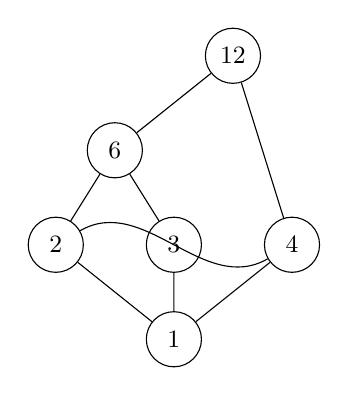
\begin{tikzpicture}[
    node distance=1.2cm,
    every node/.style={draw,circle,minimum size=0.7cm,inner sep=1pt,font=\small}
  ]
    \node (1)  at (0,0)   {$1$};
    \node (2)  at (-1.5,1.2) {$2$};
    \node (3)  at (0,1.2) {$3$};
    \node (4)  at (1.5,1.2) {$4$};
    \node (6)  at (-0.75,2.4) {$6$};
    \node (12) at (0.75,3.6) {$12$};

    \draw (1) -- (2) -- (6) -- (12);
    \draw (1) -- (3) -- (6);
    \draw (1) -- (4) -- (12);
    \draw (2) to[out=30,in=210] (4);
  \end{tikzpicture}
  \end{center}

  \item \textbf{极大/小元与最大/小元：}
  \begin{itemize}
    \item 极大元 = $\{12\}$，最大元 = $12$。
    \item 极小元 = $\{1\}$，最小元 = $1$。
  \end{itemize}

  \item \textbf{是否为格：} 是。
  在整除偏序集中，任意 $a,b\in A$，
  $\operatorname{lub}(a,b)=\operatorname{lcm}(a,b)$，
  $\operatorname{glb}(a,b)=\gcd(a,b)$。
  集合 $A=\{1,2,3,4,6,12\}$ 对最小公倍数和最大公约数封闭
  （例如 $\operatorname{lcm}(4,6)=12\in A$，
  $\gcd(4,6)=2\in A$），故 $(A,R)$ 是格。
  事实上，任意正整数的因子集在整除关系下总是格。
\end{enumerate}

\subsubsection*{Q34 \;--\; 图论综合}

\begin{enumerate}[label=(\alph*)]
  \item \textbf{Dijkstra 最短路径：}

  \medskip
  \begin{center}
  \begin{tabular}{c|c|c|c|c|c|c|c}
  \toprule
  Step & 已确定 & A & B & C & D & E & F \\
  \midrule
  0 & ---   & 0 & $\infty$ & $\infty$ & $\infty$ & $\infty$ & $\infty$ \\
  1 & A     & \textbf{0} & 4 & 2 & $\infty$ & $\infty$ & $\infty$ \\
  2 & C     & 0 & 3\;(C) & \textbf{2} & 10 & 12 & $\infty$ \\
  3 & B     & 0 & \textbf{3\;(C)} & 2 & 8\;(B) & 12 & $\infty$ \\
  4 & D     & 0 & 3\;(C) & 2 & \textbf{8\;(B)} & 10\;(D) & 14\;(D) \\
  5 & E     & 0 & 3\;(C) & 2 & 8\;(B) & \textbf{10\;(D)} & 13\;(E) \\
  6 & F     & 0 & 3\;(C) & 2 & 8\;(B) & 10\;(D) & \textbf{13\;(E)} \\
  \bottomrule
  \end{tabular}
  \end{center}

  最短路径：$A \to C \to B \to D \to E \to F$，
  长度 $= 2+1+5+2+3 = 13$。

  \item \textbf{Euler 回路/路径 与 Hamilton 回路：}

  各顶点度数：$\deg(A)=2,\; \deg(B)=3,\; \deg(C)=4,\;
  \deg(D)=4,\; \deg(E)=3,\; \deg(F)=2$
  （C 连接 A,B,D,E；D 连接 B,C,E,F）。

  \begin{itemize}
    \item \textbf{Euler 回路：} 不存在。有 2 个奇度顶点（B 和 E），
    不满足「所有顶点偶度」的充要条件。
    \item \textbf{Euler 路径：} \textbf{存在}。连通图恰有 2 个奇度顶点
    （B 和 E），满足 Euler 路径的充要条件。一条欧拉路径：
    $B \to A \to C \to B \to D \to C \to E \to D \to F \to E$。
    \item \textbf{Hamilton 回路：} 存在。$\min\deg = 2 < 6/2 = 3$，
    Dirac 条件不满足（不能保证存在），但可直接构造哈密顿回路：
    \[
    A \to B \to D \to F \to E \to C \to A.
    \]
    验证每条边均在图中：A-B($4$), B-D($5$), D-F($6$), F-E($3$), E-C($10$), C-A($2$)。
  \end{itemize}
\end{enumerate}

\subsubsection*{Q35 \;--\; Huffman 编码}

\begin{enumerate}[label=(\alph*)]
  \item \textbf{构造 Huffman 树：}

  频率（化为小数）：
  A=0.15,\; B=0.25,\; C=0.05,\; D=0.20,\; E=0.10,\; F=0.25。

  合并步骤：
  \[
  \begin{array}{ll}
  \text{Step 1} & C(0.05) + E(0.10) = CE(0.15)  \\
  \text{Step 2} & A(0.15) + CE(0.15) = ACE(0.30) \\
  \text{Step 3} & D(0.20) + F(0.25) = DF(0.45)   \\
  \text{Step 4} & B(0.25) + ACE(0.30) = BAC(0.55)\\
  \text{Step 5} & BAC(0.55) + DF(0.45) = ROOT(1.00)
  \end{array}
  \]

  构造的 Huffman 树（左枝 = 0，右枝 = 1）：

  \begin{center}
  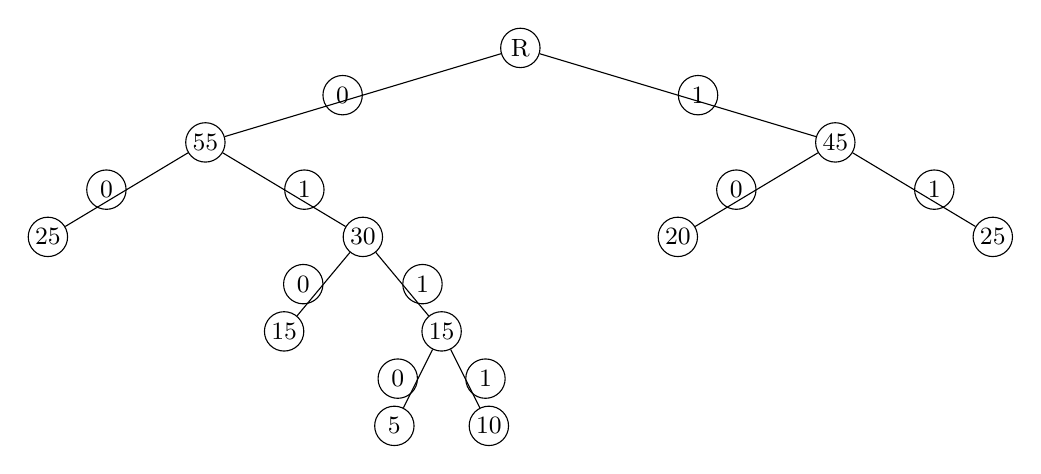
\begin{tikzpicture}[
    level distance=1.2cm,
    level 1/.style={sibling distance=8cm},
    level 2/.style={sibling distance=4cm},
    level 3/.style={sibling distance=2cm},
    level 4/.style={sibling distance=1.2cm},
    every node/.style={draw,circle,minimum size=0.5cm,inner sep=1pt,font=\small},
    edge from parent/.style={draw}
  ]
    \node (root) {R}
      child {node {55}
        child {node {25}
          edge from parent node[left] {0}
        }
        child {node {30}
          child {node {15}
            edge from parent node[left] {0}
          }
          child {node {15}
            child {node {5}
              edge from parent node[left] {0}
            }
            child {node {10}
              edge from parent node[right] {1}
            }
            edge from parent node[right] {1}
          }
          edge from parent node[right] {1}
        }
        edge from parent node[left] {0}
      }
      child {node {45}
        child {node {20}
          edge from parent node[left] {0}
        }
        child {node {25}
          edge from parent node[right] {1}
        }
        edge from parent node[right] {1}
      };
  \end{tikzpicture}
  \end{center}

  编码表：
  \begin{center}
  \begin{tabular}{c|c|c}
  \toprule
  符号 & 编码 & 长度 \\
  \midrule
  B & 00   & 2 \\
  A & 010  & 3 \\
  C & 0110 & 4 \\
  E & 0111 & 4 \\
  D & 10   & 2 \\
  F & 11   & 2 \\
  \bottomrule
  \end{tabular}
  \end{center}

  \item \textbf{平均比特数：}
  \[
  \begin{aligned}
  \text{avg} &= 2\cdot(0.25+0.20+0.25) + 3\cdot0.15 + 4\cdot(0.05+0.10)\\
            &= 2\cdot0.70 + 3\cdot0.15 + 4\cdot0.15 \\
            &= 1.40 + 0.45 + 0.60 = 2.45\ \text{bits/symbol}.
  \end{aligned}
  \]

  \item \textbf{定长编码：}
  6 个符号需要 $\lceil\log_2 6\rceil = 3$ bits/symbol。
  Huffman 编码节省了 $(3-2.45)/3 \approx 18.3\%$。
\end{enumerate}

\end{document}
